\begin{minipage}[b]{0.45\linewidth}
    \centering
    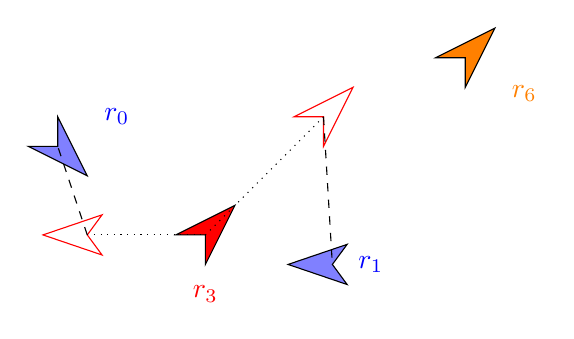
\begin{tikzpicture}[scale=1.5]
      \draw[fill=blue!50] (3,4.5) -- (2.75,5) -- (2.75,4.75) -- (2.5,4.75)   -- cycle;
      \node[color=blue] at (3.25, 5) {$r_0$};
      \draw[fill=blue!50] (5.2,3.92) -- (4.7,3.75) -- (5.2,3.58) -- (5.075,3.75)  -- cycle;
      \node[color=blue] at (5.4,3.75) {$r_1$};
      \draw[fill=red] (4,4) -- (3.75,4) -- (4.25,4.25) -- (4,3.75) -- cycle;
      \node[color=red] at (4, 3.5) {$r_3$};
      \draw[color=red] (3,4)  -- (3.125,4.17) -- (2.625,4) -- (3.125,3.83) -- cycle;
      \draw[dotted] (3,4) -- (4,4);
      \draw[color=red] (5,5) -- (4.75,5) -- (5.25,5.25) -- (5,4.75) -- cycle;
      \draw[dotted] (5,5) -- (4,4);
      \draw[dashed] (5,5) -- (5.075, 3.75);
      \draw[dashed] (3,4) -- (2.75,4.75);
      \draw[fill=orange] (6.2,5.5) -- (5.95,5.5) -- (6.45,5.75) -- (6.2,5.25)  -- cycle;
      \node[color=orange] at (6.7, 5.2) {$r_6$};
    \end{tikzpicture}
  \end{minipage}
  \begin{minipage}[b]{0.45\linewidth}
  \centering
    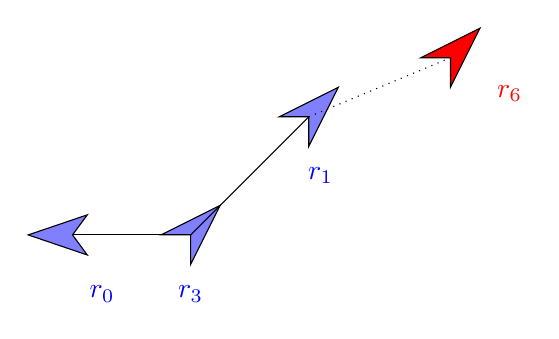
\begin{tikzpicture}[scale=1.5]
      \node[color=blue] at (3.25, 3.5) {$r_0$};
      \node[color=blue] at (5.1,4.5) {$r_1$};
      \draw[fill=blue!50] (4,4) -- (3.75,4) -- (4.25,4.25) -- (4,3.75) -- cycle;
      \node[color=blue] at (4, 3.5) {$r_3$};
      \draw[fill=blue!50] (3,4)  -- (3.125,4.17) -- (2.625,4) -- (3.125,3.83) -- cycle;
      \draw[] (3,4) -- (4,4);
      \draw[fill=blue!50] (5,5) -- (4.75,5) -- (5.25,5.25) -- (5,4.75) -- cycle;
      \draw[] (5,5) -- (4,4);
      \draw[fill=red] (6.2,5.5) -- (5.95,5.5) -- (6.45,5.75) -- (6.2,5.25)  -- cycle;
      \node[color=red] at (6.7, 5.2) {$r_6$};
      \draw[dotted] (5,5) -- (6.2,5.5);
    \end{tikzpicture}
  \end{minipage}
\caption{[left] The root robot $r_3$ assigns two positions to $r_1, r_0$, whereas robot $r_6$ is another root without any neighbor. [right] Robots $r_3, r_1, r_0$ reached assigned positions, and $r_1$ meets $r_6$ who owns the highest authority.}
